\pdfminorversion=5
\newcommand{\mytitle}{Multi-Gigabit Sub-Nyquist Sampling 60 GHz Receiver}
\newcommand{\myname}{Lorenz Koestler}
\newcommand{\myterm}{Spring Term 2014}

\documentclass[11pt, a4paper, titlepage, twoside]{book}

\usepackage[nouppercase]{scrpage2} % Kopf- und Fusszeilen formatieren
\usepackage[hang,bf]{caption}
\usepackage{ifpdf}
\usepackage[pdftex]{graphicx} \message{ETHkopf} 
\usepackage{fullpage}
\usepackage[
  colorlinks=true,        % links are colored
  citecolor=black,         % color of cite links
  %pagecolor=blue,         % color of page links
  linkcolor=black,         % color of hyperref links
  menucolor=black,         % color of Acrobat Reader menu buttons
  urlcolor=black,          % color of urls \url{}
  bookmarks=true, hyperindex=true, breaklinks=true,
  baseurl={http://www.iis.ee.ethz.ch},
  pdftitle={\mytitle},
  pdfauthor={\myname},
  pdfsubject={DFT Core generator},
  pdfkeywords={FFT, DFT, OFDM, Radix}
]{hyperref}
\usepackage[
  style=long,
  acronym,
  nonumberlist,
  numberline,
  section=chapter,
  nomain
]{glossaries} 
\usepackage[english]{babel}
\usepackage{verbatim}
\usepackage{algorithm}
\usepackage{algpseudocode}      % for algorithms
\usepackage{cite}               % will become: [2], [5]--[7]  (using cite.sty)
\usepackage{amsmath}
\usepackage{amssymb}
\usepackage{pdfpages}
\usepackage{dirtree}
\usepackage{tikz}
\usepackage{pgfplots}
\usepackage{todonotes}
\usepackage{subcaption}
\usepackage{trfsigns}

% Draft watermark
\usepackage{draftwatermark}

\makeglossaries
\makeindex

% references
\renewcommand{\eqref}[1]{(\ref{#1})}
\newcommand{\chapref}[1]{Chap.~\ref{#1}}
\newcommand{\secref}[1]{Sec.~\ref{#1}}
\newcommand{\figref}[1]{Fig.~\ref{#1}}
\newcommand{\tblref}[1]{Tbl.~\ref{#1}}
\newcommand{\appref}[1]{App.~\ref{#1}}

% Sets
\newcommand{\setN}{\mathcal{N}}

% misc. math stuff
\newcommand{\abs[1]}{\left|#1\right|}
\newcommand{\mc}[2]{\multicolumn{#1}{c|}{#2}}
   	% include standard macros

\begin{document}
\setlength{\headsep}{2ex}
\setlength{\headheight}{1.1\baselineskip}
\pagestyle{scrheadings}

% A %%%%%
\newacronym{ADC}{ADC}{Analog to Digital Converter}
\newacronym{ASIC}{ASIC}{Application-Specific Integrated Circuit}
\newacronym{AXI}{AXI}{Advanced eXtensible Interface}
\newacronym{AWG}{AWG}{Arbitrary Waveform Generator}
\newacronym{ack}{ack}{acknowledge}
% B %%%%%
\newacronym{BPSK}{BPSK}{Binary Phase-Sift Keying}
\newacronym{QPSK}{QPSK}{Quadrature Phase-Shift Keying}
% C %%%%%
\newacronym{CMOS}{CMOS}{Complementary Metal-Oxide-Semiconductor}
\newacronym{CPU}{CPU}{Central Processing Unit}
% D %%%%%
\newacronym{DDR}{DDR}{Double Data Rate}
\newacronym{DC}{DC}{Direct Current}
\newacronym{DMA}{DMA}{Direct Memory Access}
\newacronym{DAC}{DAC}{Digital to Analog Converter}
% E %%%%%    
\newacronym{ETH}{ETH}{Swiss Federal Institute of Technology}
\newacronym{EDK}{EDK}{Embedded Development Kit}
% F %%%%%
\newacronym{FFT}{FFT}{Fast Fourier Transform}
\newacronym{FPGA}{FPGA}{Field Programmable Gate Array}
\newacronym{FMC}{FMC}{FPGA Mezzanine Card}
\newacronym{FSM}{FSM}{Finite State Machine}
\newacronym{FIFO}{FIFO}{First-In, First-Out (Memory)}
% G %%%%%
% H %%%%%
% I %%%%%
\newacronym{IP}{IP}{Intellectual Property}
\newacronym{INetP}{IP}{Internet Protocol}o
\newacronym{IF}{IF}{Intermediate Frequency}
\newacronym{IO}{IO}{Input / Output}
\newacronym{IC}{IC}{Integrated Circuit}
\newacronym{ISI}{ISI}{Intersymbol Interference}
% J %%%%%
% K %%%%%
% L %%%%%
\newacronym{LVDS}{LVDS}{Low-Voltage Differential Signaling}
\newacronym{LUT}{LUT}{Lookup Table}
\newacronym{LED}{LED}{Light-Emitting Diode}
\newacronym{LSBand}{LSB}{Lower Side Band}
\newacronym{LO}{LO}{Local Oscillator}
\newacronym{LNA}{LNA}{Low-Noise Amplifier}
% M %%%%%
\newacronym{MSB}{MSB}{Most significant bit}
\newacronym{MIG}{MIG}{Memory Interface Generator}
\newacronym{MB}{MB}{Microblaze}
% N %%%%%
% O %%%%
% P %%%%
\newacronym{PCB}{PCB}{Printed Circuit Board}
\newacronym{PHY}{PHY}{Physical Layer}
\newacronym{PLL}{PLL}{Phase-Locked Loop}
% Q %%%%
\newacronym{QAM}{QAM}{Quadrature Amplitude Modulation}
% R %%%%%
\newacronym{RAM}{RAM}{Random-access Memory}
\newacronym{RF}{RF}{Radio Frequency}
\newacronym{RX}{RX}{Receiver / receive}
\newacronym{req}{req}{request}
\newacronym{RRC}{RRC}{Root-Raised-Cosine}
% S %%%%%
\newacronym{SGMII}{SGMII}{Serial Gigabit Media Independent Interface}
\newacronym{SNR}{SNR}{Signal to Noise Ratio}
% T %%%%%
\newacronym{TX}{TX}{Transmitter / transmitt}
% U %%%%%
\newacronym{USB}{USB}{Universal Serial Bus}
\newacronym{USBand}{USB}{Upper Side Band}
\newacronym{UI}{UI}{User Interface}
\newacronym{UDP}{UDP}{User Datagram Protocol}
\newacronym{UART}{UART}{Universal Asynchronous Receiver Transmitter}
% V %%%%%
% W %%%%%
% X %%%%%
% Y %%%%%
% Z %%%%%

% Add all glossary entries, even if they were not used in the text
\glsaddall

\frontmatter
\setlength{\parindent}{0pt}
\setlength{\parskip}{10pt}

\title{\mytitle}
\author{\myname}
\date{\myterm}

\begin{titlepage}
  \begin{center}

  \vspace*{-2cm}
  \begin{minipage}{\textwidth}
    
\includegraphics[width=0.6\textwidth]{ethlogo}
    \hfill
    \raggedright
    \includegraphics[width=0.3108\textwidth]{epfl}
  \end{minipage}

  \vspace{3cm}

  \begin{flushright}
    {\LARGE Master Project}\\
    \vspace{5mm}

    \href{http://tcl.epfl.ch}{Telecommunication Circuits Laboratory, EPFL}


    \vspace{1.5cm} {\LARGE \bfseries \mytitle}
    \rule{\textwidth}{0.8mm}

    \vspace{2cm}

    Lorenz Koestler $ < $\href{mailto:lorenz@koestler.ch}{lorenz@koestler.ch}$ > $ \\

    \vspace{4cm}

    \myterm

    \vspace{2cm}
    Advisors: \\
    Nicholas Preyss $ < $\href{mailto:nicholas.preyss@epfl.ch}{nicholas.preyss@epfl.ch}$ > $ \\
    Prof. Andreas Burg $ < $\href{mailto:andreas.burg@epfl.ch}{andreas.burg@epfl.ch}$ > $ \\
    Dr. Norbert Felber $ < $\href{mailto:felber@iis.ee.ethz.ch}{felber@iis.ee.ethz.ch}$ > $ \\

  \end{flushright}
\end{center}
\newpage

\end{titlepage}

\chapter*{Abstract}
During this thesis, a communication system for 60 GHz similar to the one proposed
in the \gls{IEEE} 802.11ad was implemented.
This is done to increase network throughput while
increasing the reusability of bandwidth due to the high spatial selectivity
of the 60 GHz band.
Much research was performed in increasing the throughput of communication systems
by improving spectral efficiency.
This thesis however, shows that multi-gigabit throughput is also possible using
higher, currently unused, frequency bands and high modulation schemes.
Therefor a Matlab simulation framework was written to evaluate different designs
and a \acrshort{FPGA} based evaluation platform was build to perform hardware
measurements.
It was found that hardware impairment correction is crucial for such a system
and that multi-gigabit throughput and high modulation
rates are possible.

%%  LocalWords:  IEEE reusability multi Matlab FPGA

\chapter*{Acknowledgments}
My special thank goes to my supervisors Nicholas Preyss for his great support.
He first proposed this very interesting topic, then spent many hours
teaching my everything necessary for this thesis and finally helped me when I was
stuck.
I would also like to thank Prof. Andreas Burg and everybody else of the
\gls{TCL} at \gls{EPFL} for providing the infrastructure, all the interesting
discussions and the very nice time we had during the past six months.
Finally I am very grateful to Dr. Norbert Felber, my supervisor from the
\gls{IIS} at \gls{ETHZ}, and all people in administration involved in making
this exchange possible. \\

%%  LocalWords:  Preyss Andreas TCL Felber ETHZ EPFL IIS


\tableofcontents

\mainmatter

\chapter{Introduction}
\label{ch:introduction}

\section{Motivation}
\begin{itemize}
\item Importance of mobile communication
\item Need for bigger datarates
\item Need for miniaturization
\end{itemize}

\section{60 GHz}
\begin{itemize}
\item huge bandwidth possible
\item Big delay spread
\item Phase noise
\item Big freespace attenuation
\item Possibility of small antenna arrays with many antennas
\item Almost no interferer at the moment (and later due to high attenuation)
\end{itemize}

% LocalWords:

\chapter{Theory}
\section{Image Rejection using Hilbert Filter}
\begin{itemize}
\item Can be used to sample assymetric baseband signal
\item Can be used to block mixer image
\end{itemize}

\chapter{Receiver Design}
\section{Receiver Architecture}
\subsection{Quadrature Baseband Sampling Receiver}
The most simple and
\begin{itemize}
\item Show overview picture of architecture
\item Frequency space pictures of Baseband, TX-IF, 60G, RX-IF, Baseband
\item Con: LO Self-Mixing leads to DC-Offset that has to be blocked using a
  High-Pass-Filter also removes a small part of the signal
\end{itemize}

\begin{figure}[ht]
  \centering
  \includegraphics[width=\textwidth]{figures/quad_base_rx_block_diagram}
  \caption{Block Diagram of Quadrature Baseband Sampling Receiver}
  \label{fig:rx_quad_base_bd}
\end{figure}

\subsection{Intermediate Frequency Sampling Receiver}
\begin{itemize}
\item Show overview picture of architecture
\item Frequency space pictures of Baseband, TX-IF, 60G, RX-IF, Baseband
\item RX and TX-LO offset to make sure LSB part is out of band
\end{itemize}

\begin{figure}[ht]
  \centering
  \includegraphics[width=\textwidth]{figures/if_rx_block_diagram}
  \caption{Block Diagram of Intermediate Frequency Sampling Receiver}
  \label{fig:rx_if_bd}
\end{figure}

\subsection{Quadrate Intermediate Frequency Sub-Nyquist Sampling Receiver}
\begin{itemize}
\item Show overview picture of architecture
\item Motivation: Save external mixer
\item Frequency space pictures of Baseband, TX-IF, 60G, RX-IF, Baseband
\item Sub-nyquist sampling, reference to component restrictions
\item Show how sub-nyquist sampling works with hilbert transform to generate analytical signal
\end{itemize}

\begin{figure}[ht]
  \centering
  \includegraphics[width=\textwidth]{figures/quad_if_rx_block_diagram}
  \caption{Block Diagram of Quadrate Intermediate Frequency Sub-Nyquist Sampling Receiver}
  \label{fig:rx_quad_if_bd}
\end{figure}

\section{Generation of Analytic Signal In Analog Domain}
\begin{itemize}
\item Explain how perfect analytic signal is created using hilbert transform
\item Explain how it is created using the sin/cos mixer
\item Explain error introduced in non perfect case
\end{itemize}

\chapter{Communication System and its simulation}


\begin{itemize}
\item 802.11ad oriented receiver
\item but non standard supplient
\item aim: show that big datarates are possible
\item aim: use to investigate phase noise behaviour and find other non ideal effects
\item perfomance limiting impairments
\end{itemize}

\section{Modulation and Pulse Shaping Scheme}
\begin{itemize}
\item bpsk / QAM
\item root raised cosine filter for pulse shaping
\end{itemize}


\section{Frame strucutre}
\begin{itemize}
\item 802.11ad oriented
\item ZEROS FES CES FIRST\_PES DATA PES DATA PES ... ZEROS
\item Explain reason of all fields
\item Explain cyclic properties
\end{itemize}

\section{Frequency offset estimation and correction}

\section{Phase noise estimation and correction}
\begin{itemize}
\item Cite phase noise measurements of Radoslav
\item Explain how to estimate and correct it
\item reference to own results in later chapter
\end{itemize}

\section{Simulation}
\begin{itemize}
\item General simulation flow using Matlab
\item Simulated scenarios:
  \begin{itemize}
  \item Baseband receiver
  \item Simulated 90 deg coupler using hilbert transform
  \item hardware baseband QI receiver
  \item hardware intermediate frequency QI receiver
  \end{itemize}
\item Interface to AWG
\item Interface to Oscilloscope
\item Interface to FPGA
\item Replace more and more by hardware
\end{itemize}


\chapter{FPGA}
\subsection{Overview}
\begin{itemize}
\item Block diagram of all modules and clock domains
\item Short discription of the purpose of each module
\item Some words about where more receiver functions can be added
\item Req/Ack-protocoll, everything stallable
\end{itemize}

\subsection{Clock domain planing}
\begin{itemize}
\item Reset
\end{itemize}

\subsection{Acquisition}
\begin{itemize}
\item Challenges of high speed data aquisition
\item FMC Plug
\item 4 x 12 bits ddr at 450 MHz
\item IDDR, INFIFO placement
\item Clock distribution
\item difficulties with reset 
\end{itemize}

\subsection{Storage}
\begin{itemize}
\item DDR3 and its difficulties (refresh, address scheme etc.)
\item Bandwidth calculcation (mes. numbers of datathroughput)
\item MIG of xilinx and it's userinterface
\item pitfall: Mask-Bits 
\end{itemize}

\subsection{Download}
\begin{itemize}
\item considered options: UART, Ethernet, USB2
\item Used USB-PHY and Usb2 Ip Core of xilinx
\item Microblaze software and its features
\item Implemented endpoints and the transfer protocol
\item Linux software for download
\end{itemize}

\chapter{Characterization of Components and Equipment}
\todo{add references to all datasheets of which specifiactions were taken}
\todo{add pictures}

\section{R\&S Vector Network Analyzer ZNB8}
In order to gain a deeper unserstanding of the non-idealities of the
components which were later used for the different test setups
were characterized using a Rohde \& Schwarz Vector Network Analyzer. \\

Besides the results of the measurements of which a few a presented
in the next few sections, also important lessons about measuring were
learned. It took me about one week to be able to performe meaningfull
measurements on the ZNB4 and to understand it's features.
While performing different measurements it soon became very clear then
non optimal torque while connection plugs or overbend cables
can produce notches of dozens of dBs even when using highest quality
equipment. \\

\begin{table}[h]
  \centering
  \begin{tabular}{|l|l|}
    \hline
    Frequency range & 9 kHz to 8.5 GHz \\ \hline
    Sweep speed & about 1ms for 100 points \\ \hline
    Dynamic range & up to 140 dB \\ \hline
    Power sweep range & 98 dB \\ \hline
  \end{tabular}
  \caption{Key properties of R\&S Vector Network Analyzer ZNB8}
  \label{tab:awg}
\end{table}

\section{Arbitrary waveform generator: Tektronix AWG 7122C}
\label{osec:comp_awg}

An \acrfull{AWG} was used instead of a real transmitter.
Not only because there is no transmitter available but also because of
it's flexibility. The same Matlab script used for simulations could
also call function output the baseband or the \gls{IF} signal.
The additional marker outputs could be used to trigger the oscilloscope
as well as the data acquisition process on the \gls{FPGA}.

\begin{table}[h]
  \centering
  \begin{tabular}{|l|l|}
    \hline
    Sample Rate & 12 $\text{GS}/\text{s}$, 24 $\text{GS}/\text{s}$ (interleaved) \\ \hline
    Number of analog channels & 2, 1 interleaved \\ \hline
    Analog bandwidth & 5.6 GHz \\ \hline
    Number of digital maker channels & $2 \times 2$ \\ \hline
    Vertical resoluation & 8 Bit, 10 Bit when markers are disabled \\ \hline
    Maximal waveform length & $\approx 130$ MS  \\ \hline
  \end{tabular}
  \caption{Key properties of Tektronix AWG 7122C}
  \label{tab:awg}
\end{table}

\section{58-63 GHz V-band Converter Sivers IMA FC1005V/00}
The most important is componant in the transmission chain is the
up- and downconverter from an \acrfull{IF} to the \acrfull{RF}.
For this purpose the Sivers IMA FC1005V/00 module was used.
It consists of an independent transmitt and receive path including
a horn antenna assembly, amplifiers, up-/downmixers and a pll
for frequency synthesis. It is able up-/downmix an \gls{IF}
of between 1 and 5 GHz to the \gls{RF} of 58 to 63 GHz. \\

As shown in \figref{fig:sivers} both the transmitt and receive path
use two inputs (I- and Q-channel) which are then both mixed to
\gls{RF} and than fed to a $90^\circ$ hybrid coupler. \\
This results in one of the two mirror frequency to be completely canceled
iff it of the two channel is shifted by $-90^\circ$ relative to the other.
This can be done by using another $90^\circ$ hybrid coupler working on
\gls{IF} as described in \secref{sec:comp_90deg} or by using die Hilbert
transform as shown in \todo{referenc to theory}. \\
The Sivers module is build such that it transmitts on the \gls{USBand}
(canceling the \gls{LSBand}) when the Q-channel is connected to the signal
$x(t)$ and the I-channel to $\mathcal{H}\{x(t)\}$.
\todo{describe how receiver has to be connected for LSB and double check it} \\

There are two inpepentend \gls{LO} for transmission and reception both using
the reference. There is an internal 10 MHz reference on the board. During
most measurements the reference was locked to same external reference as the
\gls{AWG} and \gls{ADC} to not have any frequency offsets when different
transmitt and receive frequencies were used.

\begin{figure}
  \centering
  \includegraphics[width=\textwidth]{figures/sivers_block_diagram}
  \caption{Block diagram of Sivers IMA FC1005V/00 Converter}
  \label{fig:sivers}
\end{figure}
\todo{add reference to siversima}

\begin{table}[h]
  \centering
  \begin{tabular}{|l|l|}
    \hline
    \acrshort{TX} and \acrshort{RX} \gls{RF} range & 58 - 63 GHz \\ \hline
    \acrshort{TX} and \acrshort{RX} \gls{IF} range & 1 - 5 GHz \\ \hline
    Saturated output power & min 16 dBm \\ \hline
    \gls{LO} leakage & typical 10 dBm, max 15 dBm \\ \hline
    \acrshort{TX} Image rejection & min 10 dB, typical 20 dB \\ \hline
    \acrshort{RX} Image rejection & min 10 dB, typical 14 dB \\ \hline
    Total Power Consumption & 9.5 W \\ \hline
  \end{tabular}
  \caption{Key properties of 58-63 GHz V-band Converter Sivers IMA FC1005V/00}
  \label{tab:awg}
\end{table}

\section{Meca 3 dB Hybrid Coupler 705S-3.000}
\label{sec:comp_90deg}

A Hybrid coupler has typically 4 ports as shown on
\figref{fig:90deg_coupler_symbol}.
One port is often 50 $\Omega$ determinated and therefor might not be connected
to a plug. \\

It is when neglacting production imperfections a fully symetric component
(inputs $x_i(t)$ with outputs $y_i(t)$ as well as indices 1 and 2
can be exchanged) and has the following relations:

\[y_1(t) = \frac{1}{\sqrt{2}} \left[x_1(t) \angle -\frac{\pi}{2} + x_2(t) \angle -\pi \right] \]
\[y_2(t) = \frac{1}{\sqrt{2}} \left[x_1(t) \angle -\pi + x_2(t) \angle -\frac{\pi}{2} \right] \]

As shown in \figref{fig:90deg_coupler_measurement} the power of
$x_1$ is not perfect equally splitted to $y_1$ and $y_2$. The power difference
is smaller than 1 db in the band from 1.8 Ghz to 4 GHz.
Also there is a little power ($\leq -20 db$) leaking from $x_1$ to $x_2$ and from
$y_1$ to $y_2$. \\

Due to missing calibration equipment the phase rotation could not be measured.
All measured numbers matched the specifications.

\begin{figure}
  \centering
  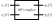
\includegraphics{figures/90deg_coupler_symbol}
  \caption{Symbol of a $90^\circ$ Coupler}
  \label{fig:90deg_coupler_symbol}
\end{figure}

\begin{figure}
  \centering
  \includegraphics[width=\textwidth]{figures/Meca_705S-3_coupler_id1}
  \caption{Measurements of Meca 3 dB Hybrid Coupler 705S-3.000,
    $x_1 \triangleq $ port 1, $y_1 \triangleq $ = port 2,
    $x_2 \triangleq $ port 3, $y_2 \triangleq $ = port 4}
  \label{fig:90deg_coupler_measurement}
\end{figure}

\begin{table}[h]
  \centering
  \begin{tabular}{|l|l|}
    \hline
    Operation range & 2 - 4 GHz \\ \hline
    Frequency Sensitivity & $\pm$ 0.4 dB \\ \hline
    Coupling variation & 3.1 dB $\pm$ 0.6 db \\ \hline
    Typical Isolation & 22 dB \\ \hline
    max VSWR & 1.2 : 1 \\ \hline
    Phase rotation & $90^\circ \pm 2.0^\circ$ \\ \hline
  \end{tabular}
  \caption{Key properties of Meca 3 dB Hybrid Coupler 705S-3.000}
  \label{tab:awg}
\end{table}

\todo{add reference}
% http://e-meca.com/rf-directional-coupler/specs_hybrid.php?ID=23&SpecsID=22#

\section{Mini-Circuits: High-Pass Filter, Amplifiers}
\begin{itemize}
\item Table with most important features
\item Show measurements done with Network Analyzer
\end{itemize}

\section{Texas-Instruments Balun ADC-WB-BB}
\begin{itemize}
\item Table with most important features
\item Show measurements done with Network Analyzer
\end{itemize}

\section{Mini-Circuits DC Block MCL BLK-89-S+}
\label{sec:comp_dc_block}
To prevent \acrshort{DC} from driving amplifier inputs into saturation
a \acrshort{DC} block was used. A significatly higher insertion loss was
measured than specified in the data sheet as shown in
\figref{fig:comp_dc_block_insertion_loss}.

\begin{table}[h]
  \centering
  \begin{tabular}{|l|l|}
    \hline
    Pass Band & 0.1 MHz to 8 GHz \\ \hline
    Specified Insertion loss up to 4 GHz & < 0.8 dB \\ \hline
    Measured Insertion loss up to 4 GHz & < 0.8 dB \\ \hline
  \end{tabular}
  \caption{Key properties of Mini-Circuits DC Block MCL BLK-89-S+}
  \label{tab:awg}
\end{table}

\begin{figure}
  \centering
  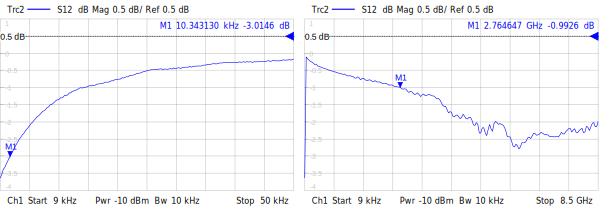
\includegraphics[width=\textwidth]{figures/MCL_BLK-89-S+_DC-Block_insertion_loss}
  \caption{Measured Insertion Loss of Mini-Circuits DC Block MCL BLK-89-S+}
  \label{fig:comp_dc_block_insertion_loss}
\end{figure}

\section{Texas Instruments ADC 12d1800}
\label{sec:comp_adc}
The receiver was build using the Ultra High-Speed ADC12D1800 by Texas Instruments.
It is able to either sample two channels at 1.8 $\text{GS}/\text{s}$ or to interleave
this two channels by applying the same input signal to both channels and sampling
one on the positive and the other one on the negative clock edge resulting in sample
rates of up to 3.6 $\text{GS}/\text{s}$. The vertical resolution of 12 bits is better
than the one of the used oscilloscope (\secref{sec:comp_osci}) and in most scenarios
not the \gls{SNR} limiting factor even when the signal is 6 db below full-scale.
The huge analog bandwidth of about 100 kHz
(limited by the \gls{DC} block described in \secref{sec:comp_dc_block}) to about
2.8 GHz allows to not only sample the first Nyquist zone but also allows
for sub-sampling which was particular interest. \\

The ADC12D1800 Reference Board was used which has a very well optimized board
layout, supports SMA plugs for all important signals, includes a \gls{FPGA}
and \gls{USB} interface for configuration and a power supply. The reference
board has an onboard \gls{PLL} but was often clocked by a marker output of the
\gls{AWG}. An \gls{FMC} connector exposes the full interface of the \gls{ADC} to
the on board \gls{FPGA} and is used by the Virtex-7 board to capture the data
as described in \chapref{chap:fpga}. \\

\begin{table}[h]
  \centering
  \begin{tabular}{|l|l|}
    \hline
    Number of channels & 2, 1 interleaved \\ \hline
    Sample Rate & $\leq$ 1.8 $\text{GS}/\text{s}$, $\leq$ 3.6 $\text{GS}/\text{s}$ interleaved \\ \hline
    Analog Bandwidth & typical 2.8 GHz \\ \hline
    Vertical Resolution & 12 bit \\ \hline
    Noise Floor Density & $\approx$ -150 $\text{dB}/\text{Hz}$ \\ \hline
    Power Consumption & 4.7 W \\ \hline
  \end{tabular}
  \caption{Key properties of Texes-Instruments ADC 12d1800}
  \label{tab:awg}
\end{table}

\section{Xilinix Virtex 7 Board VC707}
\label{sec:comp_virtex7}
\begin{itemize}
\item Table with most important features
\end{itemize}

\section{R\&S Oscilloscope RTO 1044}
\label{sec:comp_osci}
High frequency measurements were made on a Rohde \& Schwarz Digital
Oscolloscope RTO 1044. With the optional reference input it could be locked
to the \gls{AWG} as well used to have a very precise ($\pm 0.02 \text{ppm}$),
oven controlled 10 MHz reference. \\

During many experiments the real time \gls{FFT} display of the oscilloscope was
proven very usefull to check power levels and signal shapes. \\

Since the VISA standard for instrument control is painfull to install under
Redhat 6 a small programm based on the VXI-11 library written by
Steve D. Sharples \todo{reference: http://optics.eee.nottingham.ac.uk/vxi11/}
was written to convert sinmple telnet commands send by Matlab
to remote procedure calls. This allowed to setup and readout the oscilloscope
directly in the Matlab simulation framework. This was used to do first experiments
on the actual \gls{RF} hardware before the \gls{FPGA} (\chapref{chap:fpga}) was
completely implemented. \\

\begin{table}[h]
  \centering
  \begin{tabular}{|l|l|}
    \hline
    Number of channels & 4, 2 interleaved \\ \hline
    Sample Rate & 10 $\text{GS}/\text{s}$, 20 $\text{GS}/\text{s}$ interleaved \\ \hline
    Analog Bandwidth at 50 $\Omega$ & $\geq 4$ Ghz \\ \hline
    Vertical Resolution & 8 bit \\ \hline
  \end{tabular}
  \caption{Key properties of R\&S Oscilloscope RTO 1044}
  \label{tab:awg}
\end{table}

\chapter{Measurements}
\section{Narrow Band Transmission}
\label{sec:res_450}

First a relatively narrow signal transmitting at only a quarter
of the maximal symbol rate was build and analyzed to show some basic
properties of the system and to show what the best achievable
\gls{EVM} values are. \\

As receiver architecture, the Quadrature Intermediate Frequency Sub-Nyquist
Sampling Receiver as described in \secref{sec:rx_2} is used with the difference
that the signal bandwith is only $B = 450 MHz$. All the other properties are listed
in \tblref{tab:res_450}. \\

\begin{table}[h]
  \centering
  \begin{tabular}{|l|r@{}l@{~}l|}
    \hline
    $f_{\text{TX IF}}$ & 2&.9&GHz \\ \hline
    $f_{\text{TX LO}}$ & 57&.5&GHz \\ \hline
    $f_{\text{RX LO}}$ & 58&.2&GHz \\ \hline
    $f_{\text{RX IF}}$ & 2&.2&GHz \\ \hline
    $f_c$            & 60&.4&GHz \\ \hline
    Signal Bandwidth B & 0&.45&GHz \\ \hline
    Sample Rate $f_s$ & 1&.8&GHz \\ \hline
  \end{tabular}
  \caption{Properties of Narrow Band Transmission System}
  \label{tab:res_450}
\end{table}

\subsection{Measurement Setup and RF System Analysis}
A block diagram providing an overview of the test setup,
used for all following measurements, can be found in \figref{fig:res_450_bd}. \\

\begin{figure}[p]
  \centering
  %\includegraphics[width=\textwidth]{pictures/res_450_setup}
  \caption{Block Diagram of the Narrow Band Transmission Setup}
  \label{fig:res_450_bd}
\end{figure}
\todo{draw block diagram}

\begin{figure}[p]
  \centering
  %\includegraphics[width=\textwidth]{pictures/res_450_setup}
  \caption{Picture of the Narrow Band Transmission Setup}
  \label{fig:res_450_pic}
\end{figure}

\subsubsection{Matlab}
The Matlab script was configured such that it generates the transmitt signal,
programs the \gls{AWG}, reads the data acquired by the \gls{FPGA},
runs the receiver code and finally generets reports and figures. \\
The configuration file used for these tests can be found in
\appref{app:res_450_cnf}. \\

\subsubsection{\gls{AWG}}
The \gls{AWG} was configured to output the \gls{TX} \gls{IF} signal $i[k]$,
the sample clock for the \gls{ADC} as well as synchronization pulses to trigger
the \gls{FPGA} and oscillocope. It's configuration and port assignment
are shown in \tblref{tab:res_450_awg}.

It was noticed, that the used \gls{AWG} has some cross talk from
channel 1 marker 1 output to the channel 1 analog output. Therefor the
\gls{ADC} clock should always be output on marker 2 and not on marker 1.
For synchronization pulses, this is not an issue, since they are ware always
configured to give a 100 cycle wide positive pulse $> 100 \text{ns}$ before
the signal starts. \\

\begin{table}[h]
  \centering
  \begin{tabular}{|l|l|}
    \hline
    Sampling Rate & 10.8 GS/s \\ \hline
    Clock Source & Externals 10 MHz \\ \hline
    Analog Amplitude & 1 $\text{V}_{\text{pp}}$ \\ \hline
    Marker Amplitude CH1 Marker 1/2 & 0, 0.7 V \\ \hline
    Marker Amplitude CH2 Marker 1/2 & 0, 1.4 V \\ \hline
    \gls{DAC} resolution & 8 bit \\ \hline
    CH 1 & $i[k]$ \\ \hline
    CH 2 & $\mathcal{H}\{i[k]\}$ \\ \hline
    CH 1 Marker 1 & 0 \\ \hline
    CH 1 Marker 2 & 1.8 GHz \gls{ADC} sample clock \\ \hline
    CH 2 Marker 1 / 2 & Sync pulse before frame starts \\ \hline
  \end{tabular}
  \caption{Configuration and Port Assignment of \gls{AWG}}
  \label{tab:res_450}
\end{table}

An osilloscope plot (see \secref{sec:comp_osci}) of the generated
\gls{TX} \gls{IF} signal and it's \gls{FFT} can be found in
\figref{fig:res_450_awg_analog}.
The \gls{ADC} clock signal and the sync pulse are shown
in \figref{fig:res_450_awg_digital}. \\

\begin{figure}[p]
  \centering
  \includegraphics[width=\textwidth]{figures/osci/res_450_awg_analog}
  \caption{\gls{TX} \gls{IF} signal generated by the \gls{AWG}}
  \label{fig:res_450_awg_analog}
\end{figure}

\begin{figure}[p]
  \centering
  \includegraphics[width=\textwidth]{figures/osci/res_450_awg_digital}
  \caption{\gls{ADC} clock signal and sync pulse generated by the \gls{AWG}}
  \label{fig:res_450_awg_digital}
\end{figure}

\subsubsection{RF parts}
The two analog channels generated by the \gls{AWG} have a total signal
power of -9.28 dBm each \eqref{eq:res_450_awg_pwr}. These signals were
than attenuated by 20 dB to be below the 1-dB output compression point of 10 dBm
of the 60 GHz converters even at full gain of 40 dB. \\

\begin{align}
  10 \cdot \log_{10}\left(
  10^{-25.812 \;\text{dBm} / 10} \cdot
  \frac{450 \;\text{MHz}}{10 \;\text{MHz}}
  \right) \approx -9.28 \;\;\text{dBm}
  \label{eq:res_450_awg_pwr}
\end{align}

The same 60 GHz converter was used for transmission and reception and
configured as shown in \tblref{tab:res_450_sivers} (configuration script
see \appref{app:}).
A 10 MHz reference clock was fed from the \gls{AWG}.
An aluminium plate in a distance of about 15 cm was used as a reflector. \\

\begin{table}[h]
  \centering
  \begin{tabular}{|l|l|}
    \hline
    Reference Clock & external \\ \hline
    TX Oscillator Frequency & 57.5 GHz (0x038170) \\ \hline
    RX Oscillator Frequency & 58.2 GHz (0x038D60) \\ \hline
    TX Power & 0x80 \\ \hline
  \end{tabular}
  \caption{Configuration Parameters of 60 GHz Converter}
  \label{tab:res_450}
\end{table}

Both channels on the \gls{RX} side of the converer first connect to a
\gls{MC} BHP-1000+ high-pass filter. As we can see in \figref{fig:res_450_rx_if},
the \gls{TX} \gls{LO} leackage is attenuated by about 35 dB. Also the \gls{TX}
\gls{LSBand} signal (centered around 3.6 GHz) is about 17 dB weaker than
the desired \gls{TX} \gls{USBand} signal. This is due to the transmitter's
image rejection and the fact that the \gls{LSBand} signal is outside the
\gls{RF} specification of the converter. \\

\begin{figure}[p]
  \centering
  \includegraphics[width=\textwidth]{figures/osci/res_450_rx_if}
  \caption{Received \gls{IF} Signal before (left) and after (right) High-Pass Filter}
  \label{fig:res_450_rx_if}
\end{figure}p

Next the signal amplified by 12 dB to drive the \gls{ADC} input to about 70\%
as shown in \figref{fig:res_450_rx_amp}. \\

\begin{figure}[p]
  \centering
  \includegraphics[width=\textwidth]{figures/osci/res_450_rx_amp}
  \caption{Received \gls{IF} Signal before (left) and after (right) the Amplifier}
  \label{fig:res_450_rx_amp}
\end{figure}

Finally the signal is converted to a differential signal using a ADC-WB-BB Balun
(\secref{sec:comp_balun}), passes a \gls{DC} block (\secref{sec:comp_dc_block})
and digitized by the \gls{ADC}. \\

The channel filter shown in \figref{fig:rx_2_bd} is therefor build using
the BHP-1000+ high-pass filter and the \gls{ADC} analog input bandwidth which
cuts of at about 2.8 GHz. \\

\section{Error Vector Magnitude Measurements}
Random Mean Error Vector Magnitude
Deteministic Mean Error Vector Magnitude

\subsection{Channel impulse response}
\begin{itemize}
\item Show typical channel impulse response of one reflector setup.
\item Show delay spread.
\end{itemize}

\subsection{Phase Noise measurements}
\begin{itemize}
\item Phase-Noise plot measured using many short frames, show that correction algorithm works
\end{itemize}

\subsection{High Modulation Rate}
\begin{itemize}
\item Show that high modulation rates and multi GB/s throughput is possible (\gls{QAM} 256?)
\end{itemize}

\section{Full Bandwidth Transmission}
\subsection{Transmitter Channel Imbalance}
\begin{itemize}
\item Show that transmitter channel imbalance is not an issue
\end{itemize}

\subsection{90deg Coupler Error Measurement and Correction}
\begin{itemize}
\item Show error introduced by non-perfect 90 deg coupler.
\item Show the best correction I will come up with
\item Compare to best result achieved by classical architecture (with additional mixer)
\end{itemize}

%%  LocalWords:  multi QAM Coupler coupler

\chapter{Conclusion \& Outlook}
\section{Conclusion}
During the evaluation of different receiver architectures, it was found
that sub-Nyquist sampling significantly reduces the analog receiver complexity.
Using quadrature sub-Nyquist sampling gives even more flexibility in frequency
planning. \\

The chosen approach to build an \gls{FPGA} based hardware platform to get
actual measurements and using Matlab to implement all signal processing steps
in software has proven to be very efficient. The Matlab implementations
allowed for much faster development compared to implementing everything on the
\gls{FPGA}. Thereby more time was left to investigate different designs and
effects. \\

The real hardware in contrast to the simulations allowed to find
different hardware impairments like phase noise, frequency selectivity of
miscellaneous components, amplifier compression and local oscillator leakage at
mixers were found while using the hardware platform. \\

Finally it was shown, that an \gls{EVM} of -30 dB can be achieved using a channel
bandwidth of 450 MHZ, which allows for \gls{QAM}-256 modulation.
When using the full channel width of 1.8 GHz, the non-perfect
reconstruction of the analytic \gls{RX} \gls{IF} signal lead to a reduction of the
\gls{EVM} to -17 dB.

\section{Outlook}
The results suggest that the reconstruction of the analytic can be further
improved by channel estimation and correction of both samples channels
separately. This would allows to correct the different frequency selectivity
of the two outputs of the $90^\circ$ coupler shown in \secref{sec:comp_90deg}. \\

Also the implemented \gls{FPGA} design provides a good platform
for further circuit development. One could immediately start to
move receiver components, which are currently implemented in Matlab,
to programmable logic since the tricky interfaces to the \gls{ADC}
and the \gls{USB} communication with a host computer are already implemented.

%%  LocalWords:  Multi QAM Matlab FPGA Nyquist EVM coupler

\begin{appendix}
  \chapter{ADC to FPGA connections}
\label{sec:
\begin{verbatim}
NET "ID1ClkPxCI"   LOC = "L31" |IOSTANDARD = LVDS; # bank=34, byte_group=1
NET "ID1ClkNxCI"   LOC = "K32" |IOSTANDARD = LVDS; # bank=34, byte_group=1
NET "ID1PxDI[0]"   LOC = "M32" |IOSTANDARD = LVDS; # bank=34, byte_group=1
NET "ID1NxDI[0]"   LOC = "L32" |IOSTANDARD = LVDS; # bank=34, byte_group=1
NET "ID1PxDI[1]"   LOC = "W30" |IOSTANDARD = LVDS; # bank=34, byte_group=3
NET "ID1NxDI[1]"   LOC = "W31" |IOSTANDARD = LVDS; # bank=34, byte_group=3
NET "ID1PxDI[2]"   LOC = "Y29" |IOSTANDARD = LVDS; # bank=34, byte_group=3
NET "ID1NxDI[2]"   LOC = "Y30" |IOSTANDARD = LVDS; # bank=34, byte_group=3
NET "ID1PxDI[3]"   LOC = "N28" |IOSTANDARD = LVDS; # bank=34, byte_group=2
NET "ID1NxDI[3]"   LOC = "N29" |IOSTANDARD = LVDS; # bank=34, byte_group=2
NET "ID1PxDI[4]"   LOC = "R28" |IOSTANDARD = LVDS; # bank=34, byte_group=2
NET "ID1NxDI[4]"   LOC = "P28" |IOSTANDARD = LVDS; # bank=34, byte_group=2
NET "ID1PxDI[5]"   LOC = "P30" |IOSTANDARD = LVDS; # bank=34, byte_group=2
NET "ID1NxDI[5]"   LOC = "N31" |IOSTANDARD = LVDS; # bank=34, byte_group=2
NET "ID1PxDI[6]"   LOC = "R30" |IOSTANDARD = LVDS; # bank=34, byte_group=2
NET "ID1NxDI[6]"   LOC = "P31" |IOSTANDARD = LVDS; # bank=34, byte_group=2
NET "ID1PxDI[7]"   LOC = "K29" |IOSTANDARD = LVDS; # bank=34, byte_group=1
NET "ID1NxDI[7]"   LOC = "K30" |IOSTANDARD = LVDS; # bank=34, byte_group=1
NET "ID1PxDI[8]"   LOC = "J30" |IOSTANDARD = LVDS; # bank=34, byte_group=1
NET "ID1NxDI[8]"   LOC = "H30" |IOSTANDARD = LVDS; # bank=34, byte_group=1
NET "ID1PxDI[9]"   LOC = "J31" |IOSTANDARD = LVDS; # bank=34, byte_group=1
NET "ID1NxDI[9]"   LOC = "H31" |IOSTANDARD = LVDS; # bank=34, byte_group=1
NET "ID1PxDI[10]"  LOC = "L29" |IOSTANDARD = LVDS; # bank=34, byte_group=1
NET "ID1NxDI[10]"  LOC = "L30" |IOSTANDARD = LVDS; # bank=34, byte_group=1
NET "ID1PxDI[11]"  LOC = "T29" |IOSTANDARD = LVDS; # bank=34, byte_group=3
NET "ID1NxDI[11]"  LOC = "T30" |IOSTANDARD = LVDS; # bank=34, byte_group=3
NET "ID0ClkPxCI"   LOC = "K39" |IOSTANDARD = LVDS; # bank=19, byte_group=1
NET "ID0ClkNxCI"   LOC = "K40" |IOSTANDARD = LVDS; # bank=19, byte_group=1
NET "ID0PxDI[0]"   LOC = "J40" |IOSTANDARD = LVDS; # bank=19, byte_group=1
NET "ID0NxDI[0]"   LOC = "J41" |IOSTANDARD = LVDS; # bank=19, byte_group=1
NET "ID0PxDI[1]"   LOC = "P41" |IOSTANDARD = LVDS; # bank=19, byte_group=3
NET "ID0NxDI[1]"   LOC = "N41" |IOSTANDARD = LVDS; # bank=19, byte_group=3
NET "ID0PxDI[2]"   LOC = "M42" |IOSTANDARD = LVDS; # bank=19, byte_group=2
NET "ID0NxDI[2]"   LOC = "L42" |IOSTANDARD = LVDS; # bank=19, byte_group=2
NET "ID0PxDI[3]"   LOC = "H40" |IOSTANDARD = LVDS; # bank=19, byte_group=1
NET "ID0NxDI[3]"   LOC = "H41" |IOSTANDARD = LVDS; # bank=19, byte_group=1
NET "ID0PxDI[4]"   LOC = "M41" |IOSTANDARD = LVDS; # bank=19, byte_group=2
NET "ID0NxDI[4]"   LOC = "L41" |IOSTANDARD = LVDS; # bank=19, byte_group=2
NET "ID0PxDI[5]"   LOC = "K42" |IOSTANDARD = LVDS; # bank=19, byte_group=2
NET "ID0NxDI[5]"   LOC = "J42" |IOSTANDARD = LVDS; # bank=19, byte_group=2
NET "ID0PxDI[6]"   LOC = "G41" |IOSTANDARD = LVDS; # bank=19, byte_group=1
NET "ID0NxDI[6]"   LOC = "G42" |IOSTANDARD = LVDS; # bank=19, byte_group=1
NET "ID0PxDI[7]"   LOC = "M37" |IOSTANDARD = LVDS; # bank=19, byte_group=3
NET "ID0NxDI[7]"   LOC = "M38" |IOSTANDARD = LVDS; # bank=19, byte_group=3
NET "ID0PxDI[8]"   LOC = "R42" |IOSTANDARD = LVDS; # bank=19, byte_group=3
NET "ID0NxDI[8]"   LOC = "P42" |IOSTANDARD = LVDS; # bank=19, byte_group=3
NET "ID0PxDI[9]"   LOC = "N38" |IOSTANDARD = LVDS; # bank=19, byte_group=3
NET "ID0NxDI[9]"   LOC = "M39" |IOSTANDARD = LVDS; # bank=19, byte_group=3
NET "ID0PxDI[10]"  LOC = "F40" |IOSTANDARD = LVDS; # bank=19, byte_group=1
NET "ID0NxDI[10]"  LOC = "F41" |IOSTANDARD = LVDS; # bank=19, byte_group=1
NET "ID0PxDI[11]"  LOC = "R40" |IOSTANDARD = LVDS; # bank=19, byte_group=3
NET "ID0NxDI[11]"  LOC = "P40" |IOSTANDARD = LVDS; # bank=19, byte_group=3
NET "IOrPxSI"      LOC = "V30" |IOSTANDARD = LVDS; # bank=34, byte_group=3
NET "IOrNxSI"      LOC = "V31" |IOSTANDARD = LVDS; # bank=34, byte_group=3
NET "QD1ClkPxCI"   LOC = "J25" |IOSTANDARD = LVDS; # bank=36, byte_group=1
NET "QD1ClkNxCI"   LOC = "J26" |IOSTANDARD = LVDS; # bank=36, byte_group=1
NET "QD1PxDI[0]"   LOC = "H28" |IOSTANDARD = LVDS; # bank=36, byte_group=1
NET "QD1NxDI[0]"   LOC = "H29" |IOSTANDARD = LVDS; # bank=36, byte_group=1
NET "QD1PxDI[1]"   LOC = "K28" |IOSTANDARD = LVDS; # bank=36, byte_group=1
NET "QD1NxDI[1]"   LOC = "J28" |IOSTANDARD = LVDS; # bank=36, byte_group=1
NET "QD1PxDI[2]"   LOC = "G28" |IOSTANDARD = LVDS; # bank=36, byte_group=1
NET "QD1NxDI[2]"   LOC = "G29" |IOSTANDARD = LVDS; # bank=36, byte_group=1
NET "QD1PxDI[3]"   LOC = "H24" |IOSTANDARD = LVDS; # bank=36, byte_group=0
NET "QD1NxDI[3]"   LOC = "G24" |IOSTANDARD = LVDS; # bank=36, byte_group=0
NET "QD1PxDI[4]"   LOC = "K27" |IOSTANDARD = LVDS; # bank=36, byte_group=1
NET "QD1NxDI[4]"   LOC = "J27" |IOSTANDARD = LVDS; # bank=36, byte_group=1
NET "QD1PxDI[5]"   LOC = "K23" |IOSTANDARD = LVDS; # bank=36, byte_group=2
NET "QD1NxDI[5]"   LOC = "J23" |IOSTANDARD = LVDS; # bank=36, byte_group=2
NET "QD1PxDI[6]"   LOC = "G26" |IOSTANDARD = LVDS; # bank=36, byte_group=0
NET "QD1NxDI[6]"   LOC = "G27" |IOSTANDARD = LVDS; # bank=36, byte_group=0
NET "QD1PxDI[7]"   LOC = "H25" |IOSTANDARD = LVDS; # bank=36, byte_group=0
NET "QD1NxDI[7]"   LOC = "H26" |IOSTANDARD = LVDS; # bank=36, byte_group=0
NET "QD1PxDI[8]"   LOC = "H23" |IOSTANDARD = LVDS; # bank=36, byte_group=0
NET "QD1NxDI[8]"   LOC = "G23" |IOSTANDARD = LVDS; # bank=36, byte_group=0
NET "QD1PxDI[9]"   LOC = "M22" |IOSTANDARD = LVDS; # bank=36, byte_group=2
NET "QD1NxDI[9]"   LOC = "L22" |IOSTANDARD = LVDS; # bank=36, byte_group=2
NET "QD1PxDI[10]"  LOC = "K22" |IOSTANDARD = LVDS; # bank=36, byte_group=2
NET "QD1NxDI[10]"  LOC = "J22" |IOSTANDARD = LVDS; # bank=36, byte_group=2
NET "QD1PxDI[11]"  LOC = "K24" |IOSTANDARD = LVDS; # bank=36, byte_group=1
NET "QD1NxDI[11]"  LOC = "K25" |IOSTANDARD = LVDS; # bank=36, byte_group=1
NET "QD0ClkPxCI"   LOC = "E34" |IOSTANDARD = LVDS; # bank=35, byte_group=2
NET "QD0ClkNxCI"   LOC = "E35" |IOSTANDARD = LVDS; # bank=35, byte_group=2
NET "QD0PxDI[0]"   LOC = "D35" |IOSTANDARD = LVDS; # bank=35, byte_group=1
NET "QD0NxDI[0]"   LOC = "D36" |IOSTANDARD = LVDS; # bank=35, byte_group=1
NET "QD0PxDI[1]"   LOC = "E33" |IOSTANDARD = LVDS; # bank=35, byte_group=1
NET "QD0NxDI[1]"   LOC = "D33" |IOSTANDARD = LVDS; # bank=35, byte_group=1
NET "QD0PxDI[2]"   LOC = "H33" |IOSTANDARD = LVDS; # bank=35, byte_group=2
NET "QD0NxDI[2]"   LOC = "G33" |IOSTANDARD = LVDS; # bank=35, byte_group=2
NET "QD0PxDI[3]"   LOC = "F34" |IOSTANDARD = LVDS; # bank=35, byte_group=2
NET "QD0NxDI[3]"   LOC = "F35" |IOSTANDARD = LVDS; # bank=35, byte_group=2
NET "QD0PxDI[4]"   LOC = "G32" |IOSTANDARD = LVDS; # bank=35, byte_group=2
NET "QD0NxDI[4]"   LOC = "F32" |IOSTANDARD = LVDS; # bank=35, byte_group=2
NET "QD0PxDI[5]"   LOC = "G36" |IOSTANDARD = LVDS; # bank=35, byte_group=3
NET "QD0NxDI[5]"   LOC = "G37" |IOSTANDARD = LVDS; # bank=35, byte_group=3
NET "QD0PxDI[6]"   LOC = "C38" |IOSTANDARD = LVDS; # bank=35, byte_group=0
NET "QD0NxDI[6]"   LOC = "C39" |IOSTANDARD = LVDS; # bank=35, byte_group=0
NET "QD0PxDI[7]"   LOC = "J36" |IOSTANDARD = LVDS; # bank=35, byte_group=3
NET "QD0NxDI[7]"   LOC = "H36" |IOSTANDARD = LVDS; # bank=35, byte_group=3
NET "QD0PxDI[8]"   LOC = "E32" |IOSTANDARD = LVDS; # bank=35, byte_group=1
NET "QD0NxDI[8]"   LOC = "D32" |IOSTANDARD = LVDS; # bank=35, byte_group=1
NET "QD0PxDI[9]"   LOC = "H38" |IOSTANDARD = LVDS; # bank=35, byte_group=3
NET "QD0NxDI[9]"   LOC = "G38" |IOSTANDARD = LVDS; # bank=35, byte_group=3
NET "QD0PxDI[10]"  LOC = "J37" |IOSTANDARD = LVDS; # bank=35, byte_group=3
NET "QD0NxDI[10]"  LOC = "J38" |IOSTANDARD = LVDS; # bank=35, byte_group=3
NET "QD0PxDI[11]"  LOC = "B37" |IOSTANDARD = LVDS; # bank=35, byte_group=0
NET "QD0NxDI[11]"  LOC = "B38" |IOSTANDARD = LVDS; # bank=35, byte_group=0
NET "QOrPxSI"      LOC = "P25" |IOSTANDARD = LVDS; # bank=36, byte_group=3
NET "QOrNxSI"      LOC = "P26" |IOSTANDARD = LVDS; # bank=36, byte_group=3
\end{verbatim}
\end{appendix}


\appendix

\cleardoublepage
\def\acronymname{Abbreviations}
\phantomsection
\addcontentsline{toc}{chapter}{Abbreviations}
\printglossaries

\cleardoublepage
\phantomsection
\addcontentsline{toc}{chapter}{List of Figures}
\listoffigures
\listoftables\addcontentsline{toc}{chapter}{List of Tables}

\cleardoublepage
\phantomsection
\addcontentsline {toc}{chapter}{Bibliography} 
\bibliographystyle{IEEEtranS}
\bibliography{report}

\end{document}
